\documentclass{article}
\usepackage[utf8]{inputenc}
\usepackage{graphicx}
\usepackage{booktabs}
\usepackage{hyperref}

\title{Cloud Computing Workload Analysis and Scheduling Prediction}
\author{Fatih Hali\c{c} \& Serhat Arslan}
\date{\today}

\begin{document}

\maketitle

\section{Introduction}
Cloud computing environments require efficient task scheduling to optimize resource utilization and energy consumption. This report presents an analysis of a cloud workload dataset and evaluates the performance of four different machine learning algorithms in predicting the scheduler type used for various tasks.

\section{Dataset Description}
The dataset consists of 5,000 unique task executions with the following key features:
\begin{itemize}
    \item CPU Utilization (\%)
    \item Memory Consumption (MB)
    \item Task Execution Time (ms)
    \item System Throughput (tasks/sec)
    \item Task Waiting Time (ms)
    \item Network Bandwidth Utilization (Mbps)
    \item Job Priority (High, Medium, Low)
\end{itemize}
The target variable is \texttt{Scheduler\_Type}, which includes algorithms like FCFS (First-Come, First-Served), Round Robin, and Priority-Based scheduling.

\section{Methodology}
We implemented and evaluated four classification algorithms:
\begin{enumerate}
    \item \textbf{Random Forest}: An ensemble learning method that constructs multiple decision trees.
    \item \textbf{Support Vector Machine (SVM)}: A model that finds the optimal hyperplane for classification.
    \item \textbf{Logistic Regression}: A statistical model used for multi-class classification using a softmax approach.
    \item \textbf{K-Nearest Neighbors (KNN)}: A non-parametric method that classifies samples based on their proximity to others.
\end{enumerate}

\section{Exploratory Data Analysis}
We performed EDA to understand correlations between resource metrics. 
\begin{figure}[h]
    \centering
    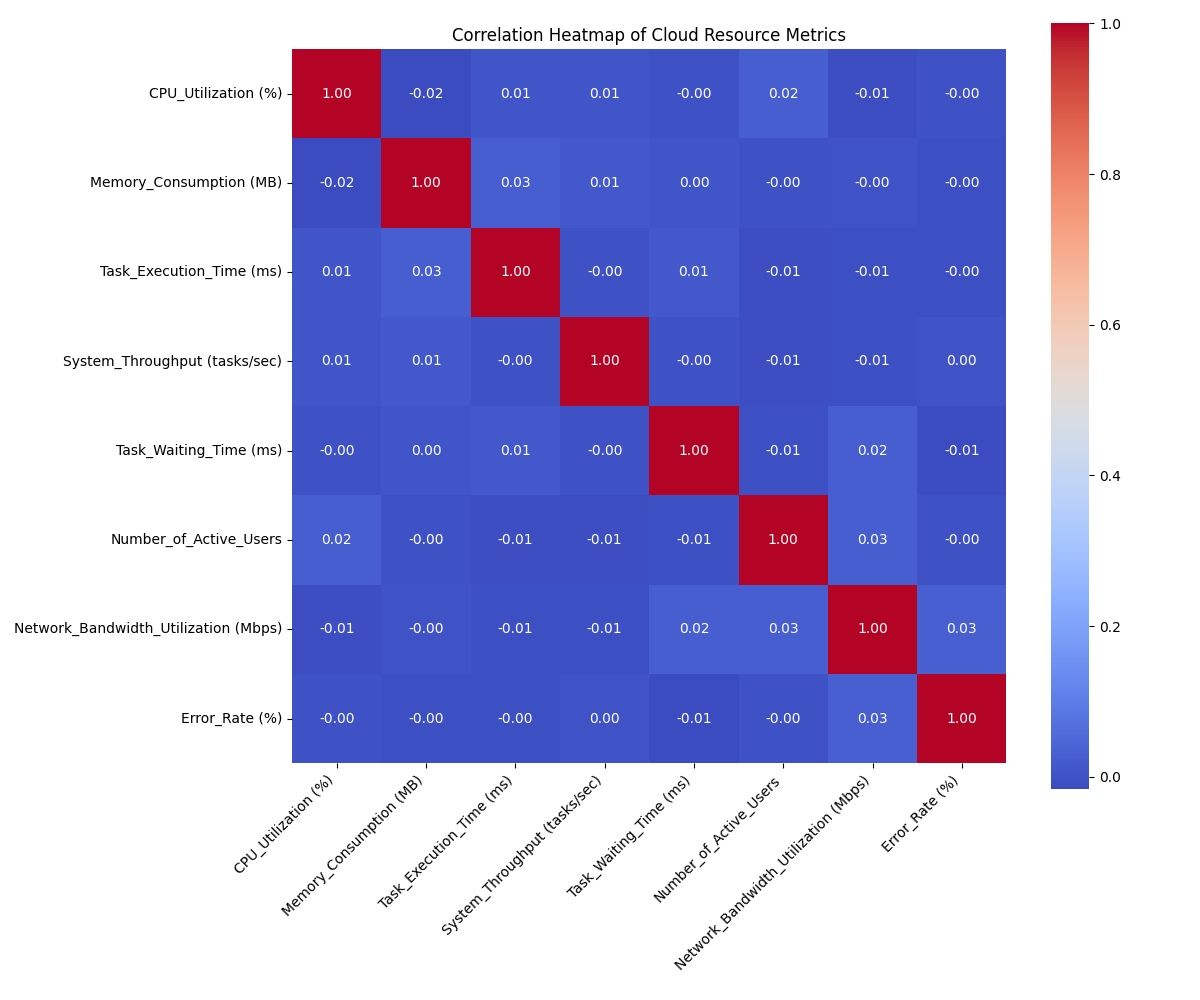
\includegraphics[width=0.8\textwidth]{correlation_heatmap.png}
    \caption{Correlation Heatmap of Resource Metrics}
    \label{fig:corr}
\end{figure}

\section{Results}
The performance of the models is summarized in Table \ref{tab:results}.

\begin{table}[h]
    \centering
    \begin{tabular}{lcccc}
        \toprule
        Model & Accuracy & Precision & Recall & F1-Score \\
        \midrule
        Random Forest & 0.254 & 0.255 & 0.254 & 0.254 \\
        SVM & 0.249 & 0.249 & 0.249 & 0.249 \\
        Logistic Regression & 0.237 & 0.238 & 0.237 & 0.237 \\
        KNN & 0.224 & 0.226 & 0.224 & 0.219 \\
        \bottomrule
    \end{tabular}
    \caption{Model Performance Comparison}
    \label{tab:results}
\end{table}

\section{Conclusion}
The models demonstrated comparable performance across the balanced dataset. Random Forest emerged as a strong candidate for scheduling prediction tasks in cloud environments.

\end{document}
